\documentclass[a4paper,12pt,oneside]{scrartcl}
\usepackage{cmap}
\usepackage[T2A]{fontenc}
\usepackage[utf8]{inputenc}
\usepackage[english]{babel}
\usepackage{textcomp}
\newcommand*{\No}{\textnumero}

\usepackage{indentfirst}

\usepackage[pdftex,
            pdfauthor={Eugene Andrienko},
            pdftitle={palm-sync-daemon description},
            pdfsubject={Technical description of palm-sync-daemon},
            pdfkeywords={Palm, OrgMode, Linux}]{hyperref}
\hypersetup{
    hidelinks,
    unicode=true,
    urlcolor=blue
}
\usepackage{breakurl}

\usepackage[fleqn]{amsmath}
\usepackage{amssymb}
\usepackage{amsfonts}
\usepackage{mathtools}
\usepackage{icomma}
\usepackage{longtable}

\usepackage{graphicx}
\graphicspath{{images/}}

\usepackage{float}
\usepackage{wrapfig}
\usepackage{afterpage}
\usepackage{paralist}
\usepackage{topcapt}
\usepackage{fancyhdr}
\usepackage{extsizes}

\usepackage{tikz}
\usepackage{pgfplots}
\usepackage{pgfplotstable}

\usepackage{listingsutf8}
\lstset{escapechar=|,
  frame=tb,
  basicstyle=\ttfamily,
  keywordstyle=\color{blue},
  commentstyle=\color{gray},
  columns=fullflexible,
  keepspaces=true,
  showstringspaces=false,
  inputencoding=utf8,
  extendedchars=true,
  captionpos=b,
  breaklines=true,
  postbreak=\raisebox{0ex}[0ex][0ex]{\ensuremath{\hookrightarrow\space}}}

\lstdefinelanguage{org}{
  keywords={TODO, VERIFIED, DONE, CANCELLED, SCHEDULED, DEADLINE},
  keywordstyle=\bfseries
}
\lstdefinelanguage{flex}{
  keywords={return},
  keywordstyle=\bfseries
}

\usepackage[backend=biber,
    abbreviate=false,
    style=alphabetic]{biblatex}
\addbibresource{bibliography.bib}


\renewcommand{\le}{\leqslant}
\renewcommand{\ge}{\geqslant}
% hm for break formulas. For ex.: \hm{=}
\newcommand{\hm}[1]{#1\nobreak\discretionary{}%
  {\hbox{$\mathsurround=0pt #1$}}{}}

\renewcommand{\thesection}{\arabic{section}.}
\renewcommand{\theequation}{\thesection\arabic{equation}}
\renewcommand{\thesubsection}{\thesection\arabic{subsection}}
\renewcommand{\labelenumii}{\theenumii}
\renewcommand{\theenumii}{\theenumi.\arabic{enumii}.}

\title{palm-sync-daemon description}
\author{Eugene Andrienko}
%\date{}


%---------------------------------------------------------------------------


\begin{document}

\clearpage
\maketitle
\thispagestyle{empty}
\newpage

\pagestyle{fancy}
\lhead{}
\chead{}
\rhead{palm-sync-daemon}
\lfoot{}
\cfoot{\arabic{page}}
\rfoot{}


\tableofcontents
\listoffigures
\listoftables
\lstlistoflistings

\newpage

\begin{tabular}{|l|l|l|}
  \hline
  \textbf{Date} & \textbf{Document version} & \textbf{Changes} \\
  \hline
  2024-01-14 & 1.0 & First version \\
  \hline
\end{tabular}

\newpage

%---------------------------------------------------------------------------

\begin{abstract}
  Main purpose of \texttt{palm-sync-daemon} is seamless synchronization between
  Palm and OrgMode files on the Linux PC. Desired goal~--- user just press
  button on the cradle (or cable) and all necessary data synchonize two way
  between Palm and OrgMode files. Without destructive changes on org-files.

  Org-files will be synchronized with the next applications on the Palm:
  \begin{itemize}
  \item Calendar
  \item Memos
  \item Tasks
  \end{itemize}

  Palm device running Palm OS 5.4.7 (Garnet).
\end{abstract}

\section{Desired OrgMode file format}
\label{sec:desired-orgmode-file}

All data from org-files divided to 3 logical parts:
\begin{enumerate}
\item Data for Memos~--- different notes, not belonging to TODO-list of calendar
  data.
\item Data for Tasks~--- tasks from TODO-list
\item Data for Calendar~--- tasks (may be repetitive) from TODO-list with time
  range.
\end{enumerate}

Lets look closer to the each type of data.

\subsection{Notes}
\label{sec:notes}

My notes stored in separate file, for example \texttt{org/notes.org}. Each note
is a first-level headline\footnote{In terms of OrgMode. See
  \url{https://orgmode.org/manual/Headlines.html}}. Under this headline can be
headlines of the next levels, some text of lists~--- all of these belongs to
the this note.

Each note can have categories or do not have categories at all. For example,
categories which I use:
\begin{itemize}
\item \texttt{doings}
\item \texttt{psychotherapy}
\item \texttt{todo}
\end{itemize}

Each note can have priority or TODO keyword\footnote{See
  \url{https://orgmode.org/manual/TODO-Basics.html}} or may not. For example, I
can use next TODO keywords:
\begin{itemize}
\item \texttt{TODO}
\item \texttt{VERIFIED}
\item \texttt{DONE}
\item \texttt{CANCELLED}
\end{itemize}

Notes example:
\begin{lstlisting}[language=org]
  * Camera wrist strap
  * Knots:
  - straight
  - figure eight
  - bowline
  - Austrian conductor
  ** From Ashley Book of Knots:
  - Knot #1119
  - Knot #5
\end{lstlisting}

\subsection{TODO-list tasks}
\label{sec:todo-list-tasks}

TODO-lists stored in a separate file. For example: \texttt{org/todo.org}. Each
TODO-list item is a first-level headline, which starts from TODO keyword
(described above).

Each TODO-list item can have a special tag:
\begin{description}
\item[mission] Small steps on the way to lifegoals.
\item[hustle] Boring but necessary things.
\item[recharge] Recreation, all what recharge <<battery>>~--- like walking,
  photography, etc.
\item[experience] Big and impressive things.
\item[routine] Everyday routine.
\end{description}

\textit{(This tags was taken from that article:
  \url{https://vas3k.club/post/24436/}).}

Or no tags at all.

Example:
\begin{lstlisting}[language=org]
  * TODO Buy bicycle parts               :recharge:
  * TODO Fix printer paper feed          :hustle:
\end{lstlisting}

Each TODO-list item \textit{may have} property \texttt{SCHEDULED} or
\texttt{DEADLINE} (with date or date+time and/or repeater interval\footnote{See
  \url{https://orgmode.org/manual/Timestamps.html}}) or just an explanatory text
right after first-level headline:
\begin{lstlisting}[language=org]
  * TODO Recall if parcel is lost
  SCHEDULED: <2024-01-02 Tue 12:00>
  Date of first call: 25-12-2023
  8-800-234-48-99
\end{lstlisting}

\subsection{Calendar tasks}
\label{sec:calendar-tasks}

Calendar tasks stored in the same file as TODO-list tasks (see
section~\ref{sec:todo-list-tasks}). But calendar tasks differs from TODO-list
tasks. Calendar tasks has a time range. Also a repeater interval may be set too.

For example:
\begin{lstlisting}[language=org]
  * TODO Therapy
  SCHEDULED: <2024-01-08 Mon 08:00-09:30 +1w>
\end{lstlisting}

\section{Synchronization process~--- first look}
\label{sec:synchr-scen-first-look}

Primarily, I want to create simple but robust synchronization algorithm. It
should neither delete data on the computer, nor lose new data coming from Palm.

Some useful information about synchronization between Palm handheld and PC can
be found in~\cite{PalmProgrammingBible}~(chapter~18: <<Building Conduits>>,
page~617). But these pieces of knowledge are not fully applicable to my case.

First, I don't archive entries neither in Emacs OrgMode, nor on Palm handheld.

Second, I cannot distinguish between edited and non-edited entries in
org-files. As you see from examples above (see
section~\ref{sec:desired-orgmode-file}), I do not store dates of creation or
modification inside drawer~--- I want my files to be visually clean.

So, to make the synchronization process robust enough, I will use \textit{three}
sources of data:
\begin{enumerate}
\item PDB files, retrieved from Palm handheld in \textit{this} synchronization
  cycle.
\item PDB files, retrieved from handheld from \textit{previous} iteration.
\item OrgMode files.
\end{enumerate}

Two sets of PDB files are necessary to determine record statuses on handheld:
\begin{longtable}[H]{|p{4cm}|p{4cm}|p{6cm}|}
  \hline
  \textbf{Record status on handheld}
  & \textbf{Record status on handheld from previous sync. iteration}
  & \textbf{Computed record status} \\
  \hline
  \hline
  No record & No record & No record \\
  \hline
  Exists & No record & Added \\
  \hline
  Exists and dirty\footnote{See about record attributes
  in~\ref{sec:pdb-header}~section.} & No record & Added \\
  \hline
  Exists and deleted & No record & No record \\
  \hline
  \hline
  No record & Exists & Deleted \\
  \hline
  Exists & Exists & Not changed \\
  \hline
  Exists and dirty & Exists & Changed \\
  \hline
  Exists and deleted & Exists & Deleted \\
  \hline
  \hline
  No record & Exists and dirty & Deleted \\
  \hline
  Exists & Exists and dirty & Not changed \\
  \hline
  Exists and dirty & Exists and dirty & Changed \\
  \hline
  Exists and deleted & Exists and dirty & Deleted \\
  \hline
  \hline
  No record & Exists and deleted & Deleted \\
  \hline
  Exists & Exists and deleted & Added \\
  \hline
  Exists and dirty & Exists and deleted & Added \\
  \hline
  Exists and deleted & Exists and deleted & Deleted \\
  \hline
  \caption{How to determine record statuses on
  handheld\label{tab:handheld-record-status}}
\end{longtable}

Computed status of handheld records and status of org-file record will be used
in synchronization logic like this:
\begin{longtable}[H]{{|p{3cm}|p{2cm}|p{9cm}|}}
  \hline
  \textbf{Computed record status from handheld}
  & \textbf{Record status in org-files}
  & \textbf{Daemon action} \\
  \hline
  \hline
  No record & No record & Do nothing \\
  \hline
  Added & No record & Add handheld record to org-files \\
  \hline
  Not changed & No record & Add handheld record to org-files \\
  \hline
  Changed & No record & Add handheld record to org-files \\
  \hline
  Deleted & No record & Do nothing \\
  \hline
  \hline
  No record & Exists & Add desktop record to handheld \\
  \hline
  Added & Exists & Copy handheld record to desktop \\
  \hline
  Not changed & Exists & Replace handheld record with desktop record \\
  \hline
  Changed & Exists & Replace desktop record with handheld record\footnote{
                     I assume, what user does not have access to PC with Emacs, when
                     using Palm PDA. And vice versa~--- user do not use Palm PDA when using PC. If
                     user changes the same record in Palm and in org-file
                     \textit{simultaneously}~--- that's \textbf{his problem}. In that case changes
                     in org-file will be lost!} \\
  \hline
  Deleted & Exists & Delete record on desktop\footnote{If user changed something
                     in org-file \textit{simultaneously} with handheld in
                     usage~--- it's changes will be lost!} \\
  \hline
  \caption{Synchronization logic\label{tab:synchronization-logic}}
\end{longtable}

\textit{Note:} dirty bit should be unset when writing PDB files back to Palm
handheld.

To match between records from Palm and from org-file I'll use next rules:
\begin{itemize}
\item Note from Palm and note in Org-file are the same if it's headers are
  equals.
\item TODO-item from Palm and TODO-item in Org-file are the same if it's header
  and (if exists) \texttt{SCHEDULED} or \texttt{DEADLINE} properties are same.
\item Calendar item from Palm and TODO-item in Org-file are the same if it's
  header and \texttt{SCHEDULED} (or \texttt{DEADLINE}) properties are same.
\end{itemize}

Because \texttt{SCHEDULED} or \texttt{DEADLINE} properties can be changed with
repeater interval~--- it should be matched not via simple string comparison. To
properly process entries with those properties~--- we should compare date-time
from handheld entry with date-time from org-file plus/minus $N$ repeater
interval. If resulting timestamps are the same~--- then corresponding properties
are the same. If properties are the same and headers of the entries are same~---
then records from handheld and in org-file are the same.

Next data will be synced between Palm PDA and org-files:

\begin{description}
\item[headline] Will be synced as headline.
\item[timestamps] Will be synced as timestamps.
\item[tags] Should be mapped to categories on the Palm. Category names should
  conform Palm Design Guidelines~\cite{PalmDesignGuide}.

  If record from org-file does not have tag~--- it should be mapped to
  \texttt{Unfilled} category on the Palm device.
\item[TODO keywords] Should be mapped in the next way:
  \begin{itemize}
  \item \texttt{TODO} and \texttt{VERIFIED} keywords maps to unchecked check-box
    on the corresponding Palm application.
  \item \texttt{DONE} and \texttt{CANCELLED} keywords should be mapped to
    checked check-box.
  \item Unchecked check-box maps to \texttt{TODO} keyword.
  \item Checked check-box maps to \texttt{DONE} keyword.
  \end{itemize}

  When synchronizing notes to the Memos application, all TODO keywords should be
  ignored.
\item[text] Any text after first-level headline (or header of record).
\end{description}

At a first approximation, I see the synchronization process as follows. User
comes home, insert Palm into the cradle and press button. After that our daemon
discovers Palm device in the system and immediately starts synchronization
process. This process runs in the background and \textbf{should not} require
user attention. Synchronization will use algorithm described in
table~\ref{tab:synchronization-logic}.

\section{Technical details}
\label{sec:technical-details}

List of libraries which used by palm-sync-daemon:

\begin{description}
\item[libpopt] Used to parse commandline options.
\item[libpisock] Used to communicate with Palm PDA. This library is a part of
  \texttt{pilot-link}
  project\footnote{\url{https://github.com/jichu4n/pilot-link/}} and can be
  installed with it.
\item[libiconv] To convert records data between UTF8 and CP1251 (used in
  FreeBSD).
\end{description}

\subsection{Processing PDB files}
\label{sec:parsing-pdb-files}

Data from Palm appilcations stored in PDB files. Binary format for application
record not specified and may vary from application to application. But header
for PDB file is standardized~\cite{PalmFileFormatSpec}.

\textbf{NB!} All mutli-byte data are big-endian.

\subsubsection{PDB header}
\label{sec:pdb-header}

All offsets in next tables are counted from the start of the file.

\begin{longtable}{|p{2cm}|p{4cm}|p{7cm}|}
  \hline
  \textbf{Offset} & \textbf{Length (bytes)} & \textbf{Description} \\
  \hline
  \texttt{0x0000} & 32 & Null-terminated string with ASCII symbols~--- name of database on the Palm PDA. \\
  \hline
  \texttt{0x0020} & 2 & Attributes \\
  \hline
  \texttt{0x0022} & 2 & Application specific version number of database \\
  \hline
  \texttt{0x0024} & 4 & Creation date (seconds from 1st January 1904 00:00:00) \\
  \hline
  \texttt{0x0028} & 4 & Modification date (seconds from 1st January 1904 00:00:00). Changed by Palm OS application when database is modified. \\
  \hline
  \texttt{0x002C} & 4 & Last backup date (seconds from 1st January 1904 00:00:00) \\
  \hline
  \texttt{0x0030} & 4 & Modification number of database \\
  \hline
  \texttt{0x0034} & 4 & Application info offset. Can be zero (NULL) \\
  \hline
  \texttt{0x0038} & 4 & Sort info offset. Can be zero (NULL) \\
  \hline
  \texttt{0x003C} & 4 & Database type identifier. Set by Palm application. \\
  \hline
  \texttt{0x0040} & 4 & Creator identifier. Usually set by Palm application to application name, all lowercase. \\
  \hline
  \texttt{0x0044} & 4 & Unique ID seed. Unique identifier set and used by Palm OS \\
  \hline
  \texttt{0x0048} & -- & Start of record list (see table~\ref{tab:record-list-format}) \\
  \hline
  \caption{PDB header format}
  \label{tab:pdb-header-format}
\end{longtable}

This file structure stored in \texttt{PDB} structure, which looks like this:
\begin{lstlisting}[language=C, caption={C structure to store PDB file contents in
    memory}]
  #define PDB_DBNAME_LEN 32

  struct PDB
  {
	char dbname[PDB_DBNAME_LEN];
	uint16_t attributes;
	uint16_t version;
	uint32_t ctime;
	uint32_t mtime;
	uint32_t btime;
	uint32_t modificationNumber;
	uint32_t appInfoOffset;
	uint32_t sortInfoOffset;
	uint32_t databaseTypeID;
	uint32_t creatorID;
	uint32_t seed;
	uint32_t nextRecordListOffset;
	uint16_t recordsQty;
	struct RecordQueue records;
	uint16_t recordListPadding;
	PDBCategories * categories;
  };
  typedef struct PDB PDB;
\end{lstlisting}

Record list has header and variable-length sequence of records. Each record is 8
byte length. In the table below there is only one record, just for example:
\begin{longtable}{|p{2cm}|p{4cm}|p{7cm}|}
  \hline
  \textbf{Offset} & \textbf{Length (bytes)} & \textbf{Description} \\
  \hline
  \texttt{0x0048} & 4 & Offset to the next record list. \textbf{Should be zero} for Palm OS 4.0 and later! \\
  \hline
  \texttt{0x004c} & 2 & Count of records \\
  \hline
  \texttt{0x004e} & 4 & Offset to record's data \\
  \hline
  \texttt{0x0052} & 1 & Record attributes \\
  \hline
  \texttt{0x0053} & 3 & Record unique ID \\
  \hline
  \caption{Record list format (one sample entry)}
  \label{tab:record-list-format}
\end{longtable}

In \texttt{PDB} structure this data stored differently. Offset to the next
record list (not used) and qty of records stored in \texttt{PDB} structure
itself. And variable list of other elements (including offset to record's data)
stored in queue\footnote{See manual page for \texttt{queue}, section~\#3. This
  is a standard part of C library.}. Elements of queue looks like this:
\begin{lstlisting}[language=C, caption={C structure to store one element of
    record from PDB file}]
  struct PDBRecord
  {
	uint32_t offset;
	uint8_t attributes;
	uint8_t id[3];
	uint64_t hash;
	void * data;
  };
  typedef struct PDBRecord PDBRecord;
\end{lstlisting}

Last two elements are just a software abstraction to simplify usage of
\texttt{PDB} structure by programmer. Field \texttt{hash} used by underlying
levels of system to match \texttt{data} fields between each other.

Field \texttt{data} stores application related data. Format depends on
application, which using specific database (PDB) on Palm.

Record attributes store the next data:
\begin{itemize}
\item First four bits (from 0 to 3) store the number of category, related to the
  record. See description of standard Palm OS categories below.
\item Last four bits (from 4 to 7) store record attributes itself (see
  page~\#605 in~\cite{PalmOSAPIRef}):
  \begin{description}
  \item[\texttt{0x10}] Secret record. Password protected.
  \item[\texttt{0x20}] Application locked access to the record. Or record can be
    changed only by Palm OS.
  \item[\texttt{0x40}] Dirty record. Set whenever user modify record data on
    Palm OS.
  \item[\texttt{0x80}] Deleted record. Set when user delete record data on Palm
    OS. Should be deleted on the next synchronization with the PC.
  \end{description}

  All record attributes can be bit OR-ed if multiple attributes are used.
\end{itemize}

End of record list may has two zero bytes after last record unique ID as
placeholder. Or more bytes, or no placeholder at all~--- so it's preferably to
navigate between PDB sections using offsets.

If application use standard Palm OS categories then application info filled by
categories info. It is standardized too:
\begin{longtable}{|p{2cm}|p{4cm}|p{7cm}|}
  \hline
  \textbf{Relative offset} & \textbf{Length (bytes)} & \textbf{Description} \\
  \hline
  \texttt{0x0000} & 2 & Renamed categories \\
  \hline
  \texttt{0x0002} & 16 & Category \#1 name (null-terminated) \\
  \hline
  \texttt{0x0012} & 16 & Category \#2 name \\
  \hline
  \texttt{0x0022} & 16 & Category \#3 name \\
  \hline
  \hline
  \texttt{0x00f2} & 16 & Category \#16 name \\
  \hline
  \texttt{0x102} & 1 & Category \#1 ID \\
  \hline
  \texttt{0x103} & 1 & Category \#2 ID \\
  \hline
  \hline
  \texttt{0x111} & 1 & Category \#16 ID \\
  \hline
  \texttt{0x112} & 1 & Last unique ID (\texttt{0x0f}) \\
  \hline
  \texttt{0x113} & 1 & Zero byte for padding \\
  \hline
  \caption{Application info with categories}
  \label{tab:application-info-categories}
\end{longtable}

There are up to 16 categories, each have 15 symbols length name plus
\texttt{'\textbackslash{}0'} at the end. If user has less categories~--- fill
corresponding fields with zeroes. Categories IDs start from zero.

Categories stored as simple structure, linked to \texttt{PDB} structure. Inside
that structure there are array of IDs and corresponding array of names inside:
\begin{lstlisting}[language=C, caption={C structure to store categories data}]
  #define PDB_CATEGORIES_STD_QTY 16
  #define PDB_CATEGORY_LEN 16

  struct PDBCategories
  {
	uint16_t renamedCategories;
	char names[PDB_CATEGORIES_STD_QTY][PDB_CATEGORY_LEN];
	uint8_t ids[PDB_CATEGORIES_STD_QTY];
	uint8_t lastUniqueId;
	uint8_t padding;
  };
  typedef struct PDBCategories PDBCategories;
\end{lstlisting}

\subsubsection{Processing Memos PDB file}
\label{sec:processing-memos-pdb}

PDB file from Memos database has the most simple format. Header is
standard~\cite{PalmFileFormatSpec}.

For example, we have next two notes with text inside and with \texttt{Unfiled}
and \texttt{Personal} categories:
\begin{figure}[H]
  \centering
  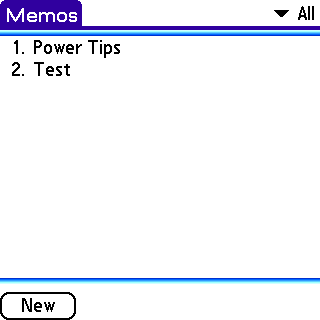
\includegraphics[width=0.5\textwidth]{memo.png}
  \caption{Sample notes in Memos application}
  \label{fig:sample-memos}
\end{figure}

For these two notes we have next binary data:

\footnotesize
\begin{verbatim}
% hexdump -C MemoDB.pdb
00000000  4d 65 6d 6f 44 42 00 00  00 00 00 00 00 00 00 00  |MemoDB..........|
00000010  00 00 00 00 00 00 00 00  00 00 00 00 00 00 00 00  |................|
00000020  00 00 00 00 e1 ce bf 5c  e1 cf 0b 83 00 00 70 80  |.......\......p.|
00000030  00 00 00 6c 00 00 00 60  00 00 00 00 44 41 54 41  |...l...`....DATA|
00000040  6d 65 6d 6f 00 00 00 00  00 00 00 00 00 02 00 00  |memo............|
00000050  01 7a 40 00 00 02 00 00  01 f0 42 56 a0 54 00 00  |.z@.......BV.T..|
00000060  00 00 55 6e 66 69 6c 65  64 00 00 00 00 00 00 00  |..Unfiled.......|
00000070  00 00 42 75 73 69 6e 65  73 73 00 00 00 00 00 00  |..Business......|
00000080  00 00 50 65 72 73 6f 6e  61 6c 00 00 00 00 00 00  |..Personal......|
00000090  00 00 00 00 00 00 00 00  00 00 00 00 00 00 00 00  |................|
*
00000160  00 00 00 01 02 00 00 00  00 00 00 00 00 00 00 00  |................|
00000170  00 00 0f 00 00 00 00 00  00 00 50 6f 77 65 72 20  |..........Power |
00000180  54 69 70 73 20 0a 95 20  49 6e 20 43 61 6c 65 6e  |Tips .. In Calen|
00000190  64 61 72 20 44 61 79 20  56 69 65 77 2c 20 70 72  |dar Day View, pr|
000001a0  65 73 73 20 4c 65 66 74  2f 52 69 67 68 74 20 6f  |ess Left/Right o|
000001b0  6e 20 74 68 65 20 6e 61  76 69 67 61 74 6f 72 20  |n the navigator |
000001c0  74 6f 20 6d 6f 76 65 20  62 61 63 6b 77 61 72 64  |to move backward|
000001d0  20 61 6e 64 20 66 6f 72  77 61 72 64 20 6f 6e 65  | and forward one|
000001e0  20 64 61 79 20 61 74 20  61 20 74 69 6d 65 2e 00  | day at a time..|
000001f0  54 65 73 74 0a 53 6f 6d  65 20 74 65 78 74 2e 2e  |Test.Some text..|
00000200  2e 00                                             |..|
\end{verbatim}
\normalsize

Here we have next data in header:
\begin{longtable}{|p{3cm}|l|l|p{5cm}|}
  \hline
  \textbf{Field} & \textbf{Offset} & \textbf{Hex value} & \textbf{Human-readable value} \\
  \hline
  Database name & \texttt{0x0000} & \texttt{4d 65 6d 6f 44 42 00} & \texttt{"MemoDB\textbackslash{}0"} \\
  \hline
  Attributes & \texttt{0x0020} & \texttt{00 00} & 0 \\
  \hline
  Version & \texttt{0x0022} & \texttt{00 00} & 0 \\
  \hline
  Creation date & \texttt{0x0024} & \texttt{e1 ce bf 5c} & 3788423004 $\Rightarrow$ 18 January 2024 11:43:24 \\
  \hline
  Modification date & \texttt{0x0028} & \texttt{e1 cf 0b 83} & 3788442499 $\Rightarrow$ 18 January 2024 17:08:19 \\
  \hline
  Last backup date & \texttt{0x002c} & \texttt{00 00 70 80} & 28800 $\Rightarrow$ 1 January 1904 10:30:17 \\
  \hline
  Modification number & \texttt{0x0030} & \texttt{00 00 00 6c} & 108 \\
  \hline
  Application info offset & \texttt{0x0034} & \texttt{00 00 00 60} & 0x60 \\
  \hline
  Sort info offset & \texttt{0x0038} & \texttt{00 00 00 00} & NULL \\
  \hline
  Database type ID & \texttt{0x003c} & \texttt{44 41 54 41} & \texttt{"DATA"} \\
  \hline
  Creator ID & \texttt{0x0040} & \texttt{6d 65 6d 6f} & \texttt{"memo"} \\
  \hline
  Unique ID seed & \texttt{0x0044} & \texttt{00 00 00 00} & 0 \\
  \hline
  \caption{PDB file header for Memos application}
  \label{tab:memos-header}
\end{longtable}

Record list contents:
\begin{longtable}{|p{3cm}|l|l|p{5cm}|}
  \hline
  \textbf{Field} & \textbf{Offset} & \textbf{Hex value} & \textbf{Human-readable value} \\
  \hline
  Next record list offset & \texttt{0x0048} & \texttt{00 00 00 00} & 0 \\
  \hline
  Count of records & \texttt{0x004c} & \texttt{00 02} & 2 \\
  \hline
  Record \#1 offset & \texttt{0x004e} & \texttt{00 00 01 7a} & \texttt{0x0000017a} \\
  \hline
  Record \#1 attributes & \texttt{0x0052} & \texttt{40} & \texttt{0x40} \\
  \hline
  Record \# unique ID & \texttt{0x0053} & \texttt{00 00 02} & \texttt{0x000002} \\
  \hline
  Record \#2 offset & \texttt{0x0056} & \texttt{00 00 01 f0} & \texttt{0x000001f0} \\
  \hline
  Record \#2 attributes & \texttt{0x005a} & \texttt{42} & \texttt{0x42} \\
  \hline
  Record \#2 unique ID & \texttt{0x005b} & \texttt{56 a0 54} & \texttt{0x56a054} \\
  \hline
  Zero bytes & \texttt{0x005e} & \texttt{00 00} & NULL \\
  \hline
  \caption{PDB file record list for Memos application}
  \label{tab:memo-record-list}
\end{longtable}

Application info (with categories):
\begin{longtable}{|p{3cm}|l|p{3cm}|p{5cm}|}
  \hline
  \textbf{Field} & \textbf{Offset} & \textbf{Hex value} & \textbf{Human-readable value} \\
  \hline
  Renamed categories & \texttt{0x0060} & \texttt{00 00} & 0 \\
  \hline
  Category \#1 & \texttt{0x0062} & \texttt{55 6e 66 69 6c 65 64 00 00 00 00 00 00 00 00 00} & Unfiled \\
  \hline
  Category \#2 & \texttt{0x0072} & \texttt{42 75 73 69 6e 65 73 73 00 00 00 00 00 00 00 00} & Business \\
  \hline
  Category \#3 & \texttt{0x0082} & \texttt{50 65 72 73 6f 6e 61 6c 00 00 00 00 00 00 00 00} & Personal \\
  \hline
  Category \#4 & \texttt{0x0092} & \texttt{00 00 00 00 00 00 00 00 00 00 00 00 00 00 00 00} & \texttt{"\textbackslash{}0"} \\
  \hline
  Category \#5 & \texttt{0x00a2} & \texttt{00 00 00 00 00 00 00 00 00 00 00 00 00 00 00 00} & \texttt{"\textbackslash{}0"} \\
  \hline
  Category \#6 & \texttt{0x00b2} & \texttt{00 00 00 00 00 00 00 00 00 00 00 00 00 00 00 00} & \texttt{"\textbackslash{}0"} \\
  \hline
  Category \#7 & \texttt{0x00c2} & \texttt{00 00 00 00 00 00 00 00 00 00 00 00 00 00 00 00} & \texttt{"\textbackslash{}0"} \\
  \hline
  Category \#8 & \texttt{0x00d2} & \texttt{00 00 00 00 00 00 00 00 00 00 00 00 00 00 00 00} & \texttt{"\textbackslash{}0"} \\
  \hline
  Category \#9 & \texttt{0x00e2} & \texttt{00 00 00 00 00 00 00 00 00 00 00 00 00 00 00 00} & \texttt{"\textbackslash{}0"} \\
  \hline
  Category \#10 & \texttt{0x00f2} & \texttt{00 00 00 00 00 00 00 00 00 00 00 00 00 00 00 00} & \texttt{"\textbackslash{}0"} \\
  \hline
  Category \#11 & \texttt{0x0102} & \texttt{00 00 00 00 00 00 00 00 00 00 00 00 00 00 00 00} & \texttt{"\textbackslash{}0"} \\
  \hline
  Category \#12 & \texttt{0x0112} & \texttt{00 00 00 00 00 00 00 00 00 00 00 00 00 00 00 00} & \texttt{"\textbackslash{}0"} \\
  \hline
  Category \#13 & \texttt{0x0122} & \texttt{00 00 00 00 00 00 00 00 00 00 00 00 00 00 00 00} & \texttt{"\textbackslash{}0"} \\
  \hline
  Category \#14 & \texttt{0x0132} & \texttt{00 00 00 00 00 00 00 00 00 00 00 00 00 00 00 00} & \texttt{"\textbackslash{}0"} \\
  \hline
  Category \#15 & \texttt{0x0142} & \texttt{00 00 00 00 00 00 00 00 00 00 00 00 00 00 00 00} & \texttt{"\textbackslash{}0"} \\
  \hline
  Category \#16 & \texttt{0x0152} & \texttt{00 00 00 00 00 00 00 00 00 00 00 00 00 00 00 00} & \texttt{"\textbackslash{}0"} \\
  \hline
  Category \#1 ID & \texttt{0x0162} & \texttt{00} & 0 \\
  \hline
  Category \#2 ID & \texttt{0x0163} & \texttt{01} & 1 \\
  \hline
  Category \#3 ID & \texttt{0x0164} & \texttt{02} & 2 \\
  \hline
  Category \#4 ID & \texttt{0x0165} & \texttt{00} & 0 \\
  \hline
  Category \#5 ID & \texttt{0x0166} & \texttt{00} & 0 \\
  \hline
  Category \#6 ID & \texttt{0x0167} & \texttt{00} & 0 \\
  \hline
  Category \#7 ID & \texttt{0x0168} & \texttt{00} & 0 \\
  \hline
  Category \#8 ID & \texttt{0x0169} & \texttt{00} & 0 \\
  \hline
  Category \#9 ID & \texttt{0x016a} & \texttt{00} & 0 \\
  \hline
  Category \#10 ID & \texttt{0x016b} & \texttt{00} & 0 \\
  \hline
  Category \#11 ID & \texttt{0x016c} & \texttt{00} & 0 \\
  \hline
  Category \#12 ID & \texttt{0x016d} & \texttt{00} & 0 \\
  \hline
  Category \#13 ID & \texttt{0x016e} & \texttt{00} & 0 \\
  \hline
  Category \#14 ID & \texttt{0x016f} & \texttt{00} & 0 \\
  \hline
  Category \#15 ID & \texttt{0x0170} & \texttt{00} & 0 \\
  \hline
  Category \#16 ID & \texttt{0x0171} & \texttt{00} & 0 \\
  \hline
  Last unique ID & \texttt{0x0172} & \texttt{0f} & 15 \\
  \hline
  Unused & \texttt{0x0173} & \texttt{00} & 0 \\
  \hline
  \caption{Application info with categories for Memos}
  \label{tab:memo-categories}
\end{longtable}

There is a strange gap between application info and notes itself~--- from
\texttt{0x0174} to \texttt{0x017a} exclusive. There are 6 bytes filled by
zeroes.

Memos format itself is simple enough. Each note starts from offset specified in
corresponding record (see table~\ref{tab:memo-record-list}). Symbols from the
start of record to first \texttt{0x0a} symbol (LF)~--- are note title. Other
symbols~--- after \texttt{0x0a} symbol to first \texttt{0x00} symbol~--- are
note contents.

Codepage for symbols is CP1251 (if you use PaPiRus cyrillic extension for Palm
OS). Otherwise there are a plain ASCII symbols.

Data format, which is used to store Memos data inside field \texttt{data} in
\texttt{PDB} structure, is simple and looks like this:
\begin{lstlisting}[language=C, caption={C structure to store memo data}]
  struct PDBMemo
  {
	char * header;
	char * text;
  };
  typedef struct PDBMemo PDBMemo;
\end{lstlisting}

\subsection{Parsing OrgMode files}
\label{sec:pars-orgm-files}

\texttt{Palm-sync-daemon} needs to parse only small subset of OrgMode syntax
(see section~\ref{sec:desired-orgmode-file}). To achieve that and do not spend a
lot of time to write own parser from zero~--- \texttt{flex} and \texttt{bison}
is used.

Tokens for OrgMode syntax is described in \texttt{src/orgmode/parser/scanner.l}:
\begin{itemize}
\item Start of first level headline
\item TODO-keyword
\item Priority
\item Tag
\item Datetime from \texttt{SCHEDULED} and \texttt{DEADLINE} directives
\item Words~--- from headline of from text below.
\end{itemize}

\begin{lstlisting}[language=flex,
  caption={Tokens, defined in \texttt{scanner.l}.},
  escapechar=]
  U             [\x80-\xbf]
  U2            [\xc2-\xdf]
  U3            [\xe0-\xef]
  U4            [\xf0-\xf4]
  UTF8SYMBOL    [[:alnum:][:punct:]]|{U2}{U}|{U3}{U}{U}|{U4}{U}{U}{U}
  TODO_KEYWORD  (TODO|VERIFIED|DONE|CANCELLED)" "
  PRIORITY      [#(A|B|C)]" "
  TAG           :[[:alnum:]]+:
  DATETIME      <[-+: [:alnum:]]+>

  %%
  ^\#\+.+\n                { /* Skip OrgMode directives */ }
  ^\*" "                   { return T_HEADLINE_STAR; }
  {TODO_KEYWORD}           { return T_TODO_KEYWORD; }
  {PRIORITY}               { return T_PRIORITY; }
  {TAG}                    { return T_TAG; }
  (SCHEDULED|DEADLINE):" " { return T_SCHEDULED; }
  {DATETIME}               { return T_DATETIME; }
  {UTF8SYMBOL}+            { return T_WORD; }
  [[:blank:]]              { /* Skip spaces */ }
  ^[\n]+                   { return T_NEWLINE; }
  [\n]                     { return T_NEWLINE; }
  %%
\end{lstlisting}

% ---------------------------------------------------------------------------

After definition of tokens, basic syntax of OrgMode is defined. See
\texttt{src/orgmode/parser/parser.y}.

\begin{lstlisting}[language=flex,
  caption={OrgMode grammar from \texttt{parser.y}.},
  escapechar=]
  %%
  entries : entry
        | T_NEWLINE entry
        | entries entry
        ;

  entry : header
      | header text
      ;

  header : headline T_NEWLINE
         | headline T_NEWLINE T_SCHEDULED T_DATETIME T_NEWLINE
         ;

  headline : T_HEADLINE_STAR line
           | T_HEADLINE_STAR line T_TAG
           | T_HEADLINE_STAR T_TODO_KEYWORD line
           | T_HEADLINE_STAR T_TODO_KEYWORD line T_TAG
           | T_HEADLINE_STAR T_PRIORITY line
           | T_HEADLINE_STAR T_PRIORITY line T_TAG
           | T_HEADLINE_STAR T_TODO_KEYWORD T_PRIORITY line
           | T_HEADLINE_STAR T_TODO_KEYWORD T_PRIORITY line T_TAG
           ;

  text : line T_NEWLINE
       | text T_NEWLINE
       | text line T_NEWLINE
       ;

  line : T_WORD
       | line T_WORD
       ;
  %%
\end{lstlisting}

Parsed OrgMode entries will be stored in next structure:
\begin{lstlisting}[language=C, caption={Structure to store OrgMode entries}]
  /**
     Priorities for OrgMode headline.

     - A - max priority
     - B
     - C - min priority
  */

  enum Priority
  {
	A,          /**< [#A] priority. */
	B,          /**< [#B] priority. */
	C,          /**< [#C] priority. */
	NO_PRIORITY /**< No priority. */
  };

  /**
     TODO-keywords for OrgMode headline.
  */
  enum TODOKeyword
  {
	TODO,
	VERIFIED,       /**< "VERIFIED" keyword. */
	DONE,           /**< "DONE" keyword. */
	CANCELLED,      /**< "CANCELLED" keyword. */
	NO_TODO_KEYWORD /**< No any of TODO-keywords. */
  };

  /**
     Repeater range - letter (h|d|w|m|y) from repeater interval.
  */
  enum RepeaterRange
  {
	HOUR,    /**< "h" letter in repeater interval. */
	DAY,     /**< "d" letter in repeater interval. */
	WEEK,    /**< "w" letter in repeater interval. */
	MONTH,   /**< "m" letter in repeater interval. */
	YEAR,    /**< "y" letter in repeater interval. */
	NO_RANGE /**< No repeater interval. */
  };

  /**
     Emacs OrgMode headline contents.

     Includes data from Flex+Bison parser. If some data is not exists in
     first-level headline - here will be NULL in corresponding field.
  */
  struct OrgModeEntry
  {
	char * header;                    /**< OrgMode first-level header */
	enum Priority priority;           /**< First-level header priority */
	enum TODOKeyword keyword;         /**< TODO-keyword for first-level header. */
	char * tag;                       /**< Tag of first-level header. May be NULL if no exists. */
	char * text;                      /**< Text below first-level header. May be NULL if no exists. */
	time_t datetime1;                 /**< Datetime or first part of time range or (time_t)-1 if no datetime. */
	time_t datetime2;                 /**< Second part of time range. May be (time_t)-1 if no time range on datetime. */
	unsigned char repeaterValue;      /**< Repeater value or 0 if no repeater interval. */
	enum RepeaterRange repeaterRange; /**< Repeater range. */
#ifndef DOXYGEN_SHOULD_SKIP_THIS
	TAILQ_ENTRY(OrgModeEntry) pointers;
#endif
  };
  #ifndef DOXYGEN_SHOULD_SKIP_THIS
  TAILQ_HEAD(OrgModeEntries, OrgModeEntry);
  typedef struct OrgModeEntry OrgModeEntry;
  #endif

  /**
     Queue of Emacs OrgMode first-level headlines.

     Contains OrgModeEntry entries.
  */
  typedef struct OrgModeEntries OrgModeEntries;
\end{lstlisting}

\subsection{Synchronization}
\label{sec:synchronization}

On the low level, synchronization process just compare hashes of records'
headers to match records from Palm PDA with records from OrgMode files. If
records' hashes matched~--- then check records' text and/or schedule, deadline
properties, tags to properly synchonize data.

As a hash-function for string I use UMASH from this repository:
\url{https://github.com/rurban/smhasher}
(see~\url{https://github.com/rurban/smhasher/blob/master/umash.h}).

\newpage

\printbibliography[heading=bibintoc]

\end{document}

%%% Local Variables:
%%% mode: latex
%%% TeX-master: t
%%% End:
